\documentclass[a4paper,12pt]{article}

\usepackage{titling}
\usepackage{float}
\usepackage{amsmath}
\usepackage{amsfonts}
\usepackage{amssymb}
\usepackage{graphicx}
\usepackage[margin=0.8in]{geometry}
\usepackage[utf8]{inputenc}

% Title information
\title{Gyroscope}
\author{Artur Topal (S5942128), Tyn Rendering (S6106366)}
\date{PUT THE DATE IN HERE}

\begin{document}

\begin{titlingpage}
  \centering
  \maketitle
  \vspace{2cm}
  \begin{abstract}
  \textit{Abstract.}
\end{abstract}

\end{titlingpage}

\break
\tableofcontents
\break
\section{Introduction} \label{sec:introduction}
A gyroscope is a device that demonstrates the interplay between angular momentum, torque, precession, and nutation. The dynamics are governed by the principles of rotational motion, which are essential for explaining the behavior of rotating systems and their applications in various scientific and engineering fields. Therefore, the aim of this report is to determine whether the precession model yields the conservation of angular momentum in the gyroscope for different external torques and initial spinning angular frequencies. The hypothesis posits that the precession frequency will increase linearly with the applied torque. This relationship can be expressed as:

\begin{equation*}
    \Omega = frac{\tao}{L}
\end{equation*}

where  is the precession frequency,  is the applied torque, and L is the angular momentum of the gyroscope. It further considers the sources of errors, as well as potential improvements to ensure more precise numerical support for the hypothesis.


\section{Theory} \label{sec:theory}
{\color{gray}\hrule}
\begin{center}
\section{Theory}
\bigskip
\end{center}
{\color{gray}\hrule}

\begin{multicols}{2}
\subsection{Introduction to general rotations}
\label{sec:theory:introduction}

Similarly to translations, there are equivalent equations for rotations:
\begin{itemize}
\item \emph{Velocity Addition} / \emph{Angular Velocity Addition}: $$\boldsymbol\omega_{1,3} = \boldsymbol\omega_{1,2} + \boldsymbol\omega_{2,3}$$
\item \emph{Momentum} / \emph{Angular Momentum}: $$\mathbf{L} = \int \mathbf{r} \times (\boldsymbol\omega \times \mathbf{r}) dm = \mathbf{I} \boldsymbol\omega$$
\item \emph{Mass} / \emph{Inertia Moment}: $$\mathbf{I} = \begin{pmatrix} I_{xx} & I_{xy} & I_{xz} \\ I_{yx} & I_{yy} & I_{yz} \\ I_{zx} & I_{zy} & I_{zz} \end{pmatrix}$$
\item \emph{Kinetic Energy}: $$T = \frac{1}{2} \boldsymbol\omega \cdot \mathbf{L} $$
\item \emph{Force} / \emph{Torque}: $$\boldsymbol\tau = \mathbf{r} \times \mathbf{F} = \frac{d\mathbf{L}}{dt} = \mathbf{I}\frac{d\boldsymbol\omega}{dt}$$
\end{itemize}

Thus, one must calculate each component in the inertia tensor ($\mathbf{I}$) depending on the coordinate system\footnote{The origin of the coordinate system is arbitrary.} to compute the net torque ($\boldsymbol{\tau}$). However, there always exists a set of principal axes\footnote{For every origin, there exists a set of principal axes} (see Section 9.3 \cite{morin}) for which all the off-diagonal components of $\mathbf{I}$ tensor are zero. Thus, $I$ reduces to $diag \begin{pmatrix} I_{xx} & I_{yy} & I_{zz} \end{pmatrix}$. There are two important consequences:
\begin{itemize}
\item $\mathbf{L}$ is aligned with the net $\boldsymbol\omega$, because the principal inertia tensor only scales $\boldsymbol\omega$.\footnote{In general, angular momentum is not collinear with angular velocity.}
\item A rigid body \emph{likes} rotating around principal axes (that is, $\boldsymbol\tau = \mathbf{0}$).
\end{itemize}

If one calculated quantities associated with rotations around CM, equations shown below relate those quantities with respect to other origins as discussed in pp. 380-383 \cite{morin}.
\begin{itemize}
\item \emph{Angular Momentum}: $\mathbf{L} = M(\mathbf{R} \times \mathbf{V}) + \mathbf{L}_{CM}$
\item \emph{Kinetic Energy}: $T = \frac{1}{2}MV^2 + \frac{1}{2}\boldsymbol\omega \cdot \mathbf{L}_{CM}$
\item \emph{Parallel-axis theorem}: $\mathbf{L} = \left( \mathbf{I}_{R} + \mathbf{I}_{CM} \right) \boldsymbol\omega$
\end{itemize}

Gyroscope consists of the homogeneous heavy cylindrical rotor of radius $R_{d}$ and mass $M_{d}$. For this lab, relevant inertia moment is calculated with respect to its symmetry axis. In cylindrical coordinates, the inertia moment is:
\begin{equation*}
  I = \int_{m}r^{2}dm = \rho\int_{0}^{H} \int_{0}^{2\pi}\int_{0}^{R_d}r^{2} rdrd\theta dz 
\end{equation*}
where
\begin{equation*}
  \rho = \frac{M_{d}}{V} = \frac{M_{d}}{\pi R_{d}^{2} H}
\end{equation*}
\begin{equation} \label{eq:theory:id}
  I = \frac{M_{d}}{\pi R_{d}^{2} H} \times H \times 2\pi \times \frac{R_{d}^{4}}{4} \Rightarrow I_{d} = \frac{1}{2} M_{d} R_{d}^{2}
\end{equation}

\subsection{Precession}
\label{sec:theory:precession}

In precession, a heavy symmetrical top (see figure \ref{fig:theory:top}) keeps a constant angle $\theta$ with the vertical $\hat{z}$ by rotating around this axis with angular velocity $\boldsymbol\Omega = \Omega \hat{z}$, and spinning around its symmetry axis $\hat{x_{3}}$ with angular velocity $\boldsymbol\omega_{3} = \omega_{3} \hat{x_{3}}$. Since a heavy symmetric top is symmetrical around $\hat{x_{3}}$, this axis is its principal axis. All other axes (e.g., $\hat{x_{2}}$ and $\hat{x_{1}}$) orthogonal to $\hat{x_{3}}$ are also principal if the origin lies on the $\hat{x_{3}}$ axis (see Section 9.6 and Section 9.3 Theorem 9.5-9.6 \cite{morin} for more details).

\begin{figure}[H]
  \centering
  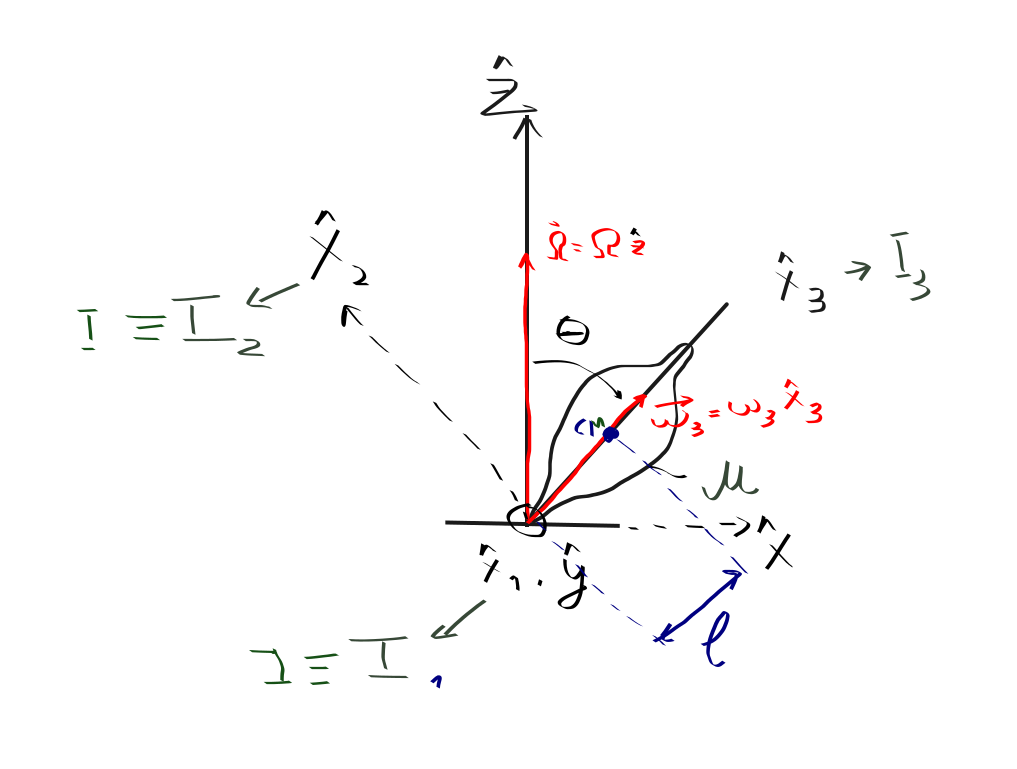
\includegraphics[width=\columnwidth]{gyroscope/images/top}
  \caption{A heavy symmetrical top}
  \label{fig:theory:top}
\end{figure}

For the system in figure \ref{fig:theory:top}, the precession frequency $\Omega$ and the spinning $\omega$ are related by (see Section 9.7 \cite{morin} for derivation):
\begin{equation*}
  \Omega_{\pm} = \frac{I_{3}\omega_3}{2I\cos(\theta)} \left( 1 \pm \sqrt{1 - \frac{4MIgl\cos(\theta)}{I_{3}^{2} \omega_{3}^{2}}}  \right)
\end{equation*}
where
\begin{itemize}
\item $I$: inertia moment of the heavy symmetric top around $\hat{x_{2}}$ or $\hat{x_{1}}$ ($I_{1} = I_{2} = I$)
\item $I_{3}$: inertia moment of the heavy symmetric top around $\hat{x_{3}}$
\item $M$: mass of the top
\item $l$: distance from the pivot to CM of the top
\end{itemize}

However, in this lab report an approximate relation for large $\omega_{3}$ is used.
\begin{equation}
  \label{eq:theory:precession_frequency}
  \Omega \approx \frac{Mgl}{I_{3}\omega_{3}}
\end{equation}

Then, precession period is
\begin{equation}
  \label{eq:theory:precession_period}
  T_{p} = \frac{2\pi}{\Omega} = \frac{2\pi I_{3} \omega_3}{Mgl} = \frac{4\pi^{2} I_{3}}{MglT_{3}}
\end{equation}
where $\omega_{3} = \frac{2\pi}{T_{3}}$.

\subsection{Nutation}
\label{sec:theory:nutation}

Nutation is a phenomenon where $\theta$ is not constant but it fluctuates around some value with angular velocity $\omega_{n}$. Since nutation is often coupled with precession, the top precesses in an ellipse around $\hat{z}$ axis. Nutation angular velocity $\omega_{n}$ and $\theta$ are given by:
\begin{equation}
  \label{eq:theory:nutation_frequency}
  \omega_{n} = \frac{I_{3}\omega_3}{I}
\end{equation}
\begin{equation*}
  \theta(t) = B + (\frac{A}{\omega_n}\sin \theta_{0})\cos(\omega_{n}t + \gamma), \left\{ A, B, \theta_{0}, \gamma \right\} \subset \mathbb{R}
\end{equation*}

\end{multicols}


\section{Methods} \label{sec:methods}
{\color{gray}\hrule}
\begin{center}
\section{Methods} \label{sec:methods}
\end{center}
{\color{gray}\hrule}

\begin{multicols}{2}
The goal of this experiment was to investigate how the angular velocity and applied torque influence the precession behavior of the gyroscope. The experimental setup, shown in Figure 1, consists of a rotating disc mounted on a low-friction axis with two degrees of freedom. To balance the gyroscope, removable counterweights were used. The TISensorTag sensor was mounted on the vertical axis and was used in conjunction with the Phyphox app to measure the angular velocity.

\begin{figure}[H]
    \centering
    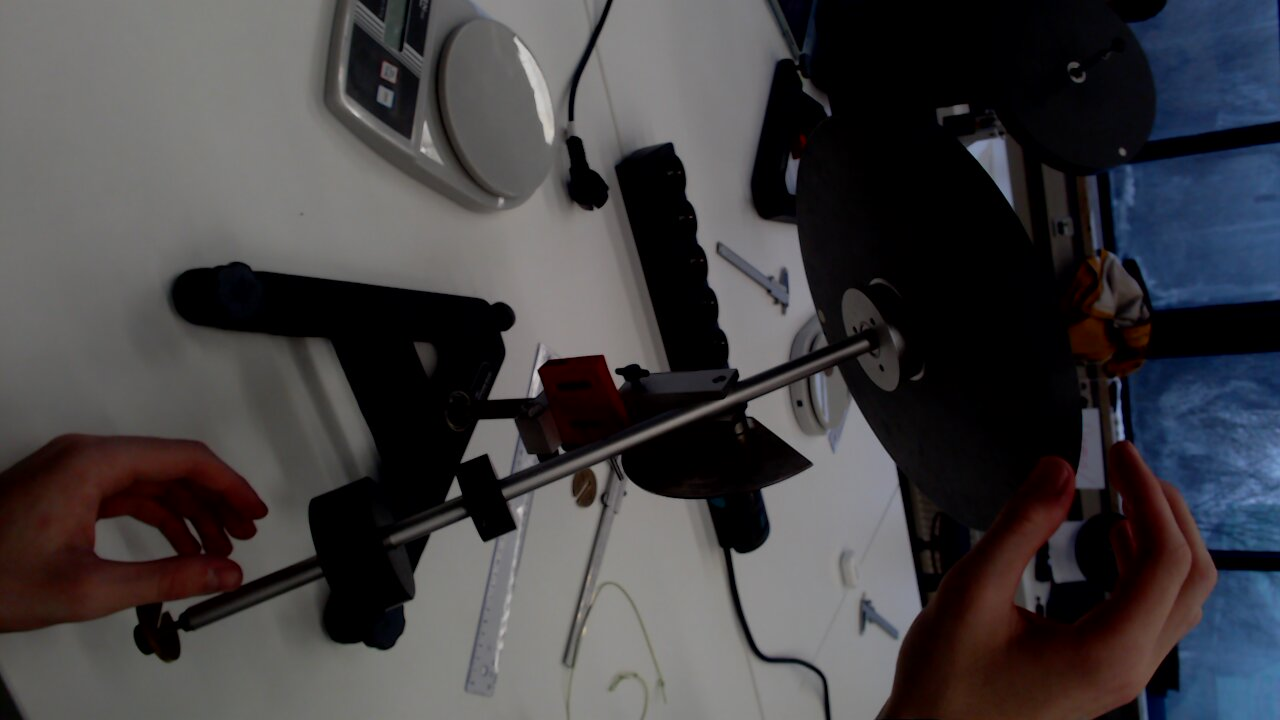
\includegraphics[width=\columnwidth]{gyroscope/images/setup}
    \caption{Placeholder}
    \label{setep}
\end{figure}

The experiment began with balancing the gyroscope by adjusting the counterweights so no torque was exerted in its free configuration. Once balanced, the rotor disc was manually started. In the first phase of the experiment, the natural behavior of the gyroscope was determined.
In the second phase, torque was applied by placing one or two weights at one end of the rotor axis. The distance between the vertical axis and the center of mass of the weights was measured. The weights were removed and attached at the other end of the rotor axis and the distance was again measured. 
In the third phase, the gyroscope was set in motion, and its behavior was recorded using a digital camera operating at x frames per second to determine the rotor’s time of revolution. These measurements were repeated for the two weight positions to analyze precession behavior under varying torque conditions.
For each part of the experiment x amount of measurements were taken to minimize random errors.

\end{multicols}


\section{Results} \label{sec:results}
{\color{gray}\hrule}
\begin{center}
\section{Results} \label{sec:results}
\bigskip
\end{center}
{\color{gray}\hrule}

\begin{multicols}{2} 
The mass of the weights were calculated using digital weights: $M = 29.9 \pm 0.1 (g)$.
\begin{equation} \label{eq:results:weight}
  \left\langle M \right\rangle = \frac{1}{N}\sum\limits_{i=1}^{N}M_{i} = 29.9 (g)
\end{equation}
\begin{equation} \label{eq:results:weight_err}
  \Delta M = \frac{1}{N}\sqrt{\sum\limits_{i=1}^{N}(M_{i} - \left\langle M \right\rangle)^{2}} = 0.1 (g)
\end{equation}

As discussed in section \ref{sec:discussion}, weights were attached to either ends of the gyroscope. However, weight's position was pushed towards the gyroscope vertical axis due to rotations (see figure \ref{fig:results:locs}). Three possible locations were measured using vernier callipers to be:
\begin{equation*}
  \left\langle l_{I} \right\rangle = \frac{1}{N}\sum\limits_{i=1}^{N}l_{Ii} = 33.0 (cm)
\end{equation*}
\begin{equation*}
  \Delta l_{I} = \frac{1}{N}\sqrt{\sum\limits_{i=1}^{N}(l_{Ii} - \left\langle l_{I} \right\rangle)^{2}} = 0.4 (cm)
\end{equation*}

Thus, $l_{I} = 33.0 \pm 0.4 (cm)$. Similarly, $l_{II} = 19.7 \pm 0.1 (cm)$ and $l_{III} = 23.9 \pm 0.1 (cm)$.

\emph{TISensorTag} was recording precession frequency ($\boldsymbol\Omega$) of the gyroscope (vertical axis) for different torques\footnote{Torque is specified by the mass of the weight and the lever arm length where the weight was attached with respect to the vertical axis of the gyroscope.} and different spinning angular velocities $\boldsymbol\omega_{3}$. This data is shown in table \ref{tab:results:precession} for each point (see appendix \ref{sec:appendix:precession_raw_data} for more details about precession frequency data, and appendix \ref{appendix:errors} for detailed error analysis).

\end{multicols}

\begin{table}[H]
  \centering
  \begin{tabular}{|c|c|c|c|c|}
    Point & Type & Precession ($\boldsymbol\Omega$), $\frac{rad}{s}$ & Mass ($M$), $g$ & Lever Arm Length ($l$), $cm$ \\ \hline
    $\#1$ & $II$ & $0.449711 \pm 0.031443$ & $59.8 \pm 0.2$ & $19.7 \pm 0.1$ \\ \hline
    $\#2$ & $II$ & $0.716604 \pm 0.055174$ & $59.8 \pm 0.2$ & $33.0 \pm 0.4$ \\ \hline
    $\#3$ & $II$ & $0.18821 \pm 0.02623$   & $29.9 \pm 0.1$ & $23.9 \pm 0.1$ \\ \hline
    $\#4$ & $II$ & $0.56268 \pm 0.06639$   & $59.8 \pm 0.2$ & $33.0 \pm 0.4$ \\ \hline
    $\#5$ & $I$  & $0.528033 \pm 0.005273$ & $29.9 \pm 0.1$ & $33.2 \pm 0.4$ \\ \hline
    $\#6$ & $I$  & $0.258233 \pm 0.002976$ & $29.9 \pm 0.1$ & $33.2 \pm 0.4$ \\ \hline
    $\#7$ & $I$  & $0.165118 \pm 0.000843$ & $59.8 \pm 0.2$ & $19.7 \pm 0.1$ \\ \hline
  \end{tabular}
  \caption{Precession frequencies ($\Omega$)}
  \label{tab:results:precession}
\end{table}

\begin{multicols}{2}
In the first part of the experiment the rotor’s behavior without external forces was observed, for this the rotor was rotated by hand. After this the base was rotated, during the rotation of the base the rotor remained stationary. This is caused by conservation of angular momentum. Angular momentum conservation also explains why it is only possible to throw a flat object over a long distance if it has spin; a spinning object resists changes in its orientation, this stabilizes the object's flight and keeps it flat, reducing wobbling.
\begin{figure}[H]
  \centering
  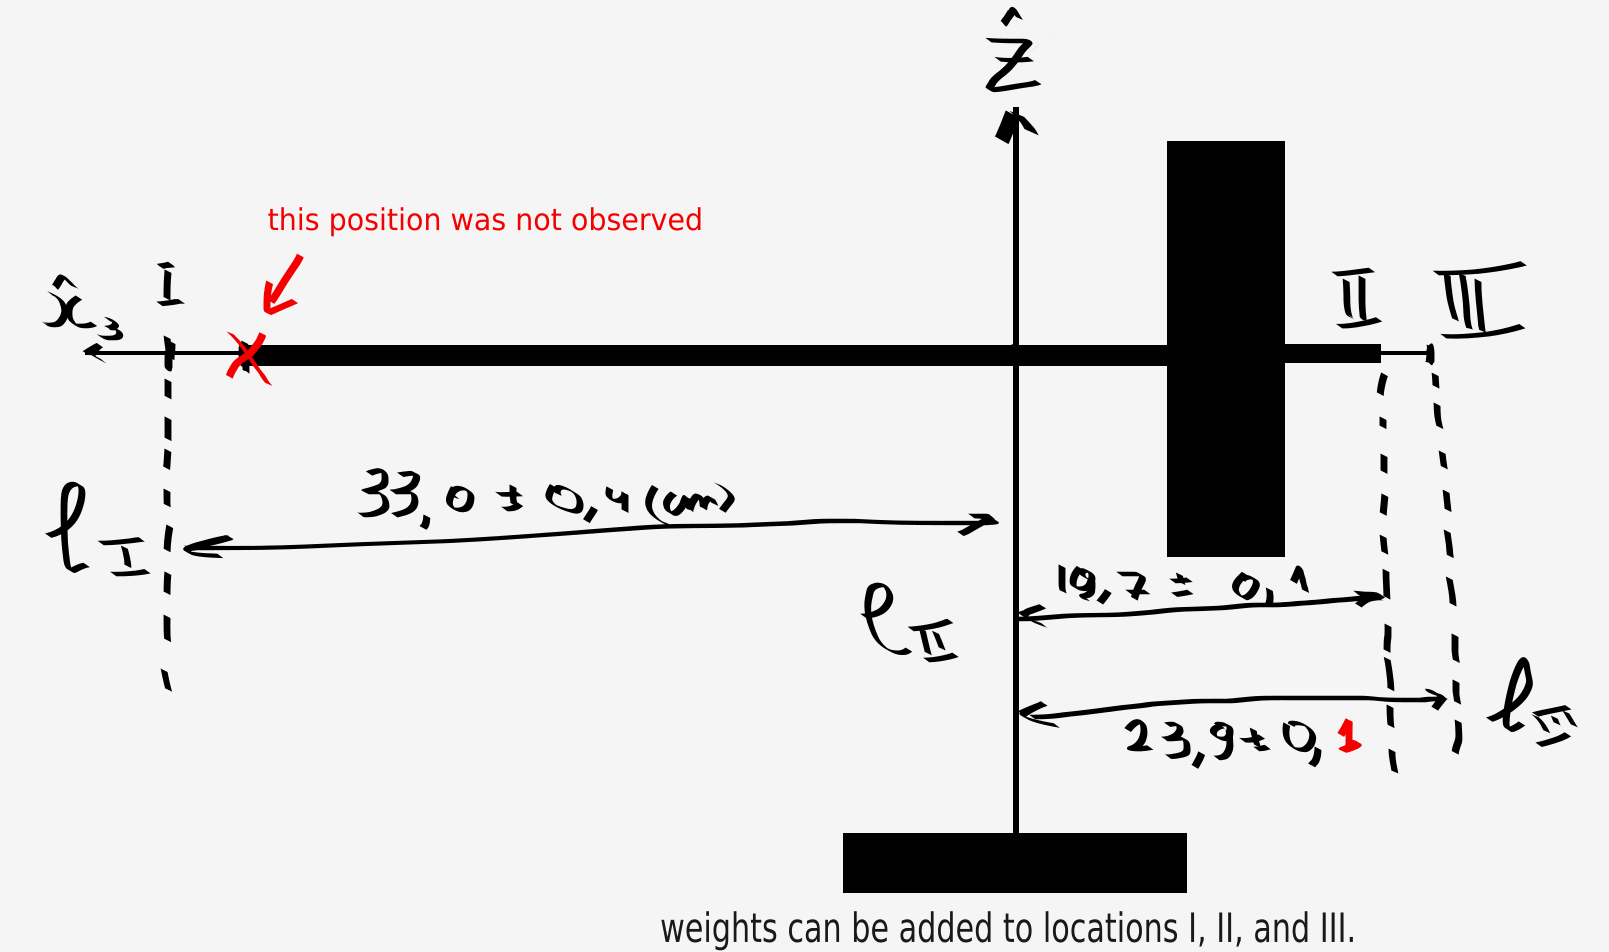
\includegraphics[width=\columnwidth]{gyroscope/images/locs}
  \caption{Possible weights locations on the gyroscope's rotor axis. }
  \label{fig:results:locs}
\end{figure}

The gyroscope would only precess if a torque was applied to it, this was done by adding weights to the setup. The weight had a mass of $29.9 \pm 0.1 (g)$ (see equation \ref{eq:results:weight} and \ref{eq:results:weight_err}), the masses were placed at distances of $l_{I}$, $l_{II}$ and $l_{III}$ from the vertical axis of the gyroscope.
Next the moment of inertia of the rotor around its own axis was determined, this was done using equation \ref{eq:theory:id}.
where $M_d = 1.74 (kg)$ is the mass of the rotor disc and $R_d = 12.47 \pm 0.04 (cm)$ is the radius of the disc. Substituting in the values of $M_d$ and $R_d$ gave $I_3 = 0.0271 \pm 0.0004 (kg \cdot m^2)$. After this, $T_3$ was calculated by the following equation:
\begin{equation*}
    T_3 = \frac{10}{A_{r}}
\end{equation*}
Where $A_{r}$ is the average rotaions per 10 seconds, which was determined by filming the setup an dividing the film in $10$ second long clips, counting the rotations per clip and then taking the average. The differnt values of $T_3$ are shown in Table x in the appendix. The previous measured components were used to calculate $T_{p, \text{calculated}}$ using equation \ref{eq:theory:precession_period}. $T_{p, \text{measured}}$ was calculated using:
\begin{equation*}
    T_{p, \text{measured}} = \frac{2\pi}{\Omega}
\end{equation*}
$T_{p, \text{calculated}}$ was plotted against $T_{p, \text{measured}}$ in figure \ref{fig:gyro}.

\begin{figure}[H]
    \centering
    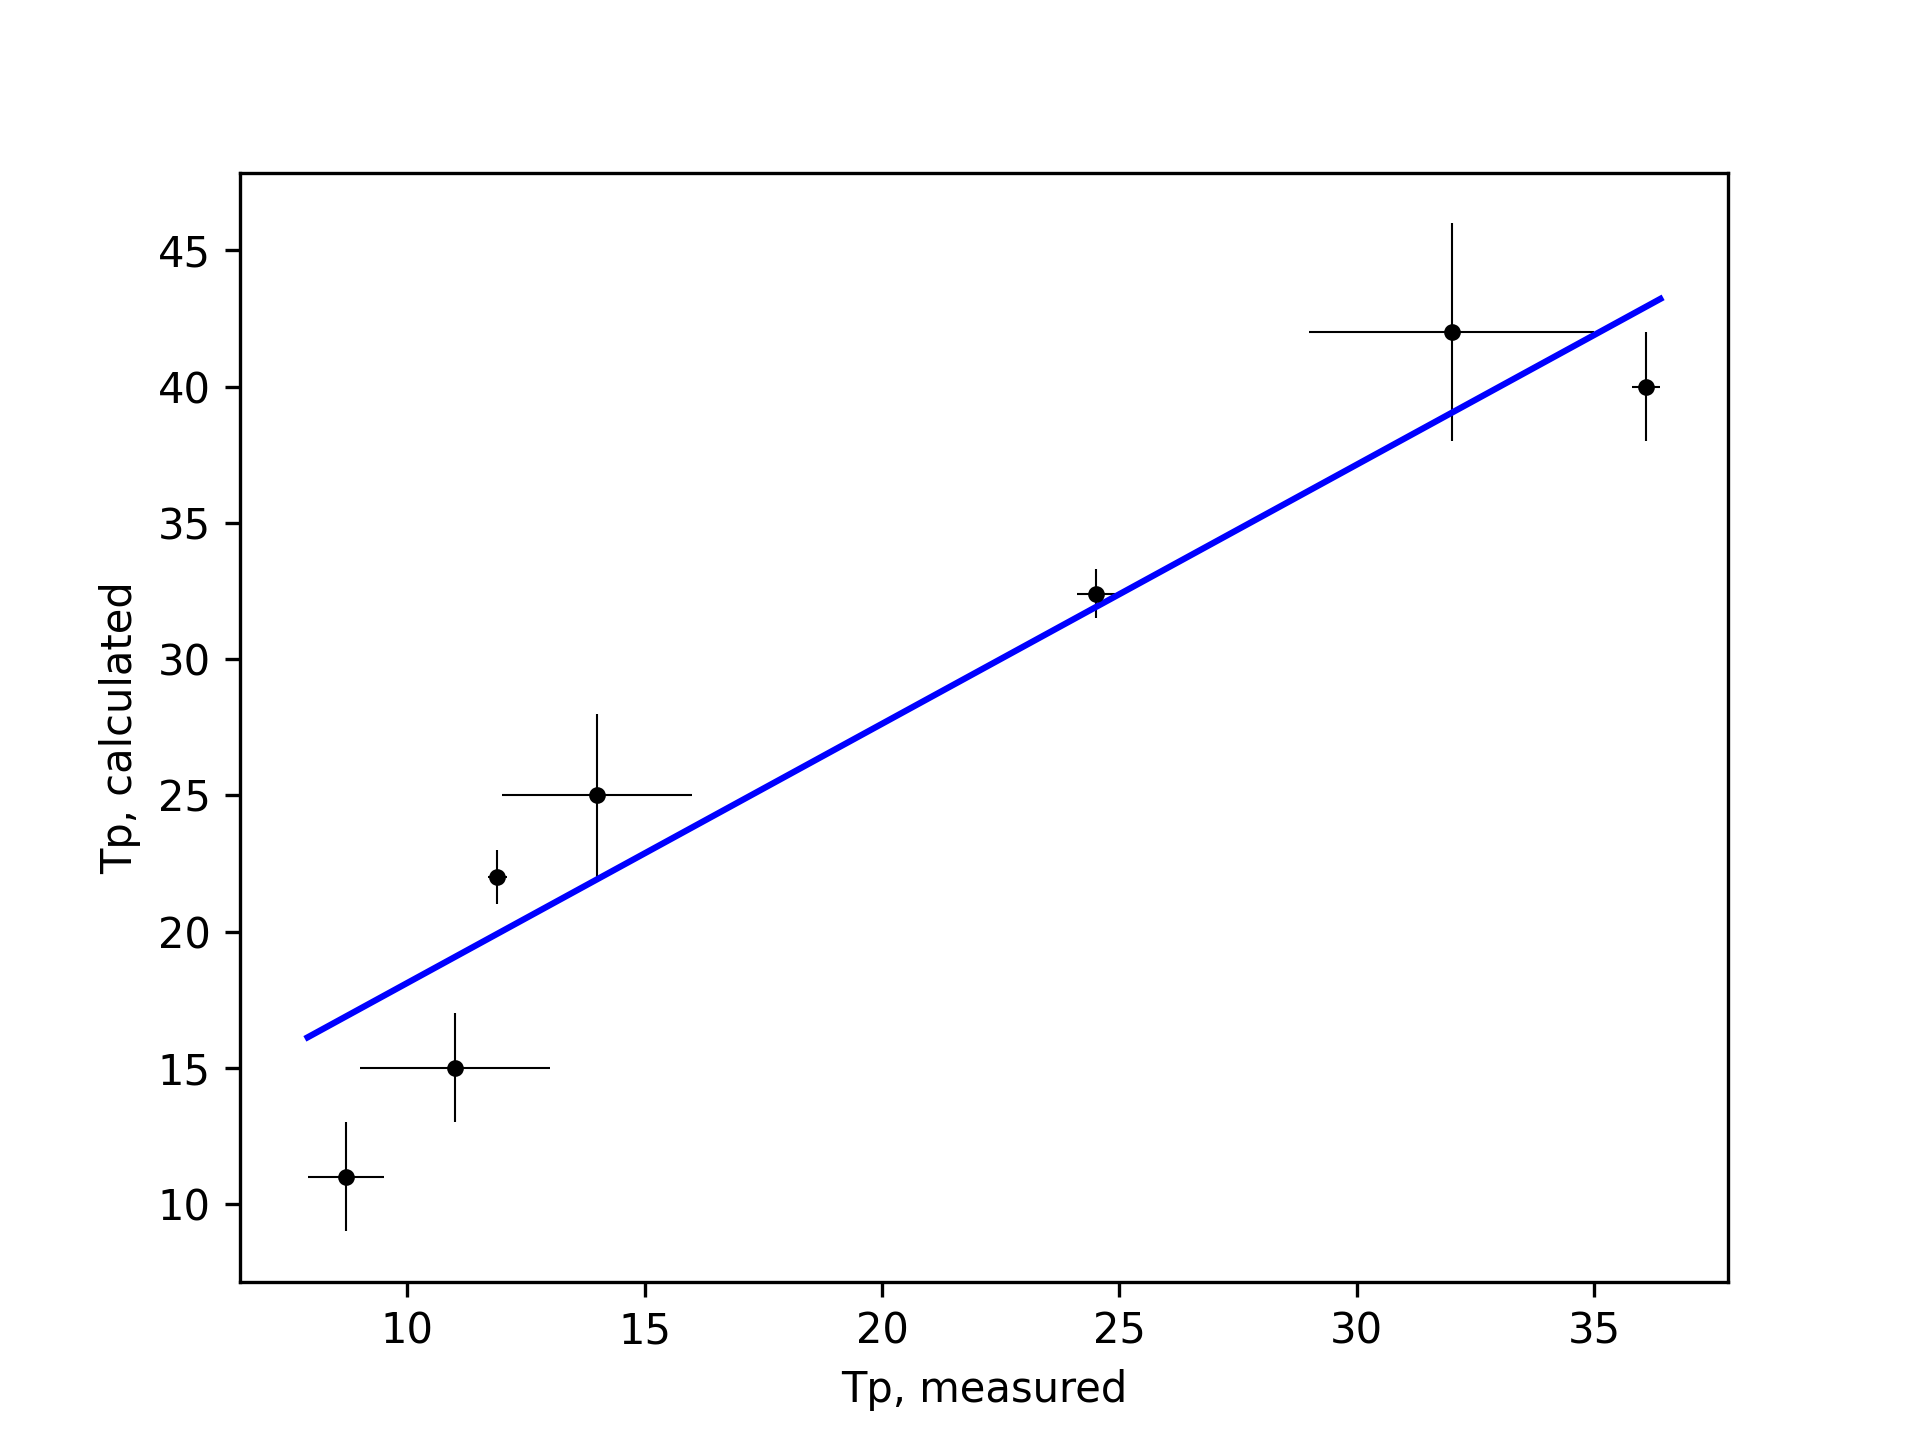
\includegraphics[width=\columnwidth]{gyroscope/images/gyro}
    \caption{Correlation between calculated and measured precession periods}
    \label{fig:gyro}
\end{figure}

The line of best fit has a slope of
\begin{equation}
  \label{eq:results:slope}
  \Delta \theta = 1.0 \pm 0.2 (rad)
\end{equation}

\end{multicols}


\section{Discussion} \label{sec:discussion}
{\color{gray}\hrule}
\begin{center}
\section{Discussion} \label{sec:discussion}
\bigskip
\end{center}
{\color{gray}\hrule}

\begin{multicols}{2}
\subsection{No external forces}
\label{sec:discussion:no}

In the beginning of the experiment, no external forces were being exerted on the gyroscope, and the motion of its rotor axis was observed upon gentle tilting or rotation of the base\footnote{Tilting or rotating in such a way that the rotor axis does not experience any external torque.}. The rotor axis maintained its spatial orientation with respect to an inertial frame (e.g., the table's frame of reference). This resistivity is based on the conservation of angular momentum ($\vec{L} = \mathbf{I}\vec{\omega} = const$) when no external torques are applied. Because the angular momentum vector remained constant in orientation and magnitude, and $\hat{x}_{3}$ rotor axis is the principal axis of the gyroscope, its spinning angular velocity ($\boldsymbol\omega_{3}$) is aligned with the angular momentum. Thus, the spinning angular velocity ($\boldsymbol\omega_{3}$) also maintains its orientation and magnitude.

\begin{figure}[H]
  \centering
  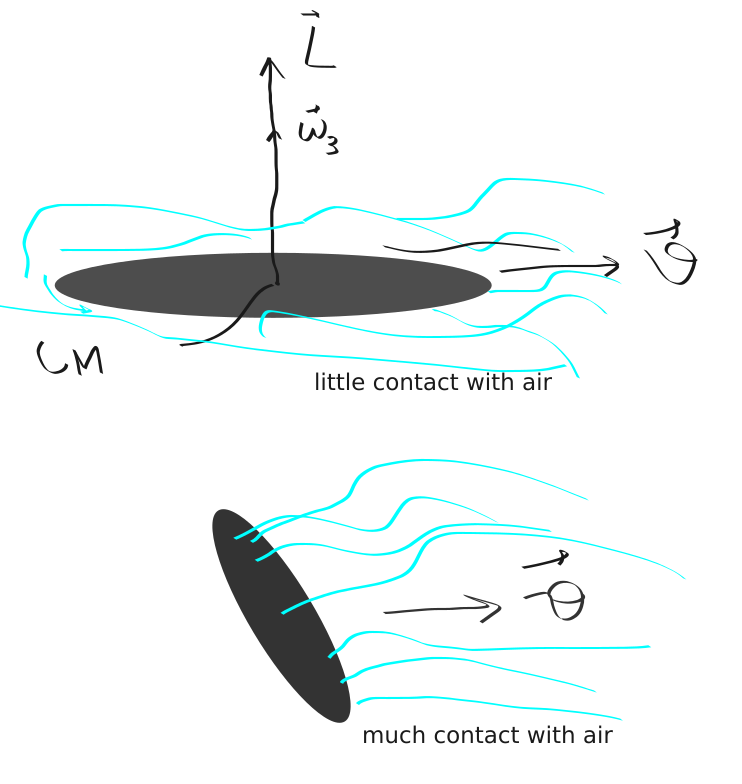
\includegraphics[width=0.7\columnwidth]{gyroscope/images/thin}
  \caption{Aerodynamics of a thin object }
  \label{fig:discussion:thin}
\end{figure}

Notably, this phenomenon explains why it is possible to throw a regularly shaped, thin object (e.g., a frisbee or discus) over longer distances if it is given a spin rather than if it is not rotating. Achieving long-distance transportation requires stability and sufficient airodynamic properties to resist air resistivity. If the object is given a spin around its center of mass as shown in figure \ref{fig:discussion:thin}, its angular momentum is conserved during flight in the absence of external torques. This conservation counteracts air's random force fluctuations on the object's surface, maintaining its aerodynamic orientation (i.e.,the thin face aligned in the direction of motion). Consequently, this object will travel over longer distances. Conversely, if no spinning is applied, random force fluctuations in air on the object surface will deorient and destabilize the object, effectively reducing its aerodynamic properties. Thus, this object will not travel as far due to higher air resistivity. 

\subsection{Comparison between $T_{p, \text{calculated}}$ and $T_{p, \text{measured}}$}

The plot of $T_{p, \text{calculated}}$ versus $T_{p, \text{measured}}$ yields the line of best fit with the slope of $1.0 \pm 0.2$. This suggests a linear relationship between the calculated and measured precession periods, which is consistent with the theoretical predictions and is a strong evidence to support the validity of the precession model.
However, for most of the points in figure \ref{fig:gyro} it is the case that the line of best fit does not fall within their uncertainties, there is also a large variation between the size of the uncertainties per datapoint. The uncertainties can be attributed to a combination of random and systematic error, the random errors mostly consisted of fluctuations in angular velocity, which could not be precisely replicated with pulling on the string by hand. As for systematic errors, they arose from frictional forces.

\subsection{Improvements} \label{sec:discussion:improvements}

An insufficient number of processed precession frequencies ($\Omega$) and corresponding spinning periods ($T_{3}$) significantly affected the error in the calculation of the slope (see result \ref{eq:results:slope}). Additionally, certain aspects of the gyroscope setup introduced deviation from the theoreical ideal case:

1. The vertical axis of the gyroscope was not perfectly aligned, resulting in a slight tilt.

2. During the gyroscope's motion, both the counterweights and torque-introducing weights experienced small linear displacement relative to the roto's axis accelerating frame of reference.

3. The initial spinning frequency ($\omega_{3}$) and the attachment of counterweights were set and adjusted by eye, which inherently introduced human error. This error was big for the initial spinning frequencies ($\omega_{3}$).

In order to calculate the precession period $T_{p_{calculated}}$ accurately, many precession frequency samples were required for each measurement\footnote{Each measurement has the same magnitude of the initial spinning angular frequency ($\omega_{3}$) and the applied torque (mass-lever-arm couple)}. However, since the initial spinning angular frequency was imparted by manually pulling a string wrapped around the rotor's reel, it was impossible to ensure consistency in torque and spinning frequency for each sample per measurement. This introduced significant uncertainty in $\omega_{3}$ accross measurements.

Moreover, pure precession of the gyroscope was not always achieved. In many instances, nutation was observed during the motion. The following actions were taken in response to this:

1. If nutation diminished over time, the dataset was trimmed to retain only the segment coressponding to pure precession.

2. If nutation persisted, mean precession frequency was estimated (see section \ref{sec:theory:nutation}).

In either case, nutation established noise in data, leading to bigger uncertainty in the precession frequencies ($\Omega$).

Finally, the spinning period ($T_{3}$) was calculated by manually estimating the time needed to make a full revolution (see \ref{sec:methods}) and evaluating the mean and the mean squared error. This manual calculation brought in a big error in the spinning period ($T_{3}$).

To improve the accuracy of the slope and strengthen the foundation for the research question of this lab report, the following steps are recommended. First, a digital motor controlled by software can be used to launch and maintain the rotor. This would ensure a precise, constant, and controlled initial spinning angular velocities for each sample per every measurement. Besides, videos of the spinning of the rotor can be fed into a neural network capable of feature extracting (e.g., see \cite{nn}). Neural network extracts the spinning period ($T_{3}$) with a much higher accuracy. Alternatively, a separate sensor can be placed in the precessing frame of reference that would measure the spinning period during the course of the sample's motion. Lastly, counterweights and torque-introducing weights should be set in-place using, for instance, nails protruding through the rotory axis. The locations for all weights should be estimated using computer techniques.   
\end{multicols}


\section{Conclusions} \label{sec:conclusions}
{\color{gray}\hrule}
\begin{center}
\section{Conclusion}
\bigskip
\end{center}
{\color{gray}\hrule}

\begin{multicols}{2}
  \lipsum{1}
\end{multicols}


% Perhaps, we will need \appendix

\end{document}
